\chapter{\texttt{meteR}: An R package for testing the Maximum Entropy Theory of Ecology}

{\large Andrew J. Rominger and Cory Merow}
\vspace{3.5em}

\noindent
In revision for \textit{Methods in Ecology and Evolution}

\clearpage

\noindent
\textbf{Abstract}
\vspace{\baselineskip}

\begin{enumerate}
\item Macroecological patterns appear to follow consistent forms
  across a range of natural systems, however the origin of their
  regularity remains obscured. The Maximum Entropy Theory of Ecology
  (METE) predicts macroecological patterns of abundance, metabolic
  rates and their distribution within communities and across space
  using an information theoretic approach. METE's success in
  predicting empirical patterns demands that we further press the
  theory's predictions to determine how (or whether) predictability
  depends on attributes of the system and the temporal, spatial and
  biological scales at which we study it.
%
\item METE predicts multiple macroecolgical metrics using statistical
  idealizations from information theory; thus confronting METE with
  data represents a strong test of the underlying biological
  mechanisms that could drive real communities away from statistical
  idealizations. METE has remained somewhat inaccessible due to its
  highly mathematical nature and a lack of software for model
  construction/evaluation. To remedy this, we have developed an
  \texttt{R} package implementation of METE.
%
\item Our open source (GNU General Public License v2) \texttt{R} package,
  \texttt{meteR} (version 1.0;
  \texttt{cran.r-project.org/web/packages/meteR}), (1) directly
  calculates
  all of METE's predictions from a variety of data formats; (2)
  automatically handles approximations and other technical details;
  (3) provides high-level plotting and model comparison functions to
  explore and interrogate models. 
%
\item With these tools in hand, ecologists can more readily test the
  predictions of METE for their data sets. By facilitating tests of
  METE, we expect that a better understanding of its strengths and
  limitations will emerge. A better understanding of the strengths and
  limitations of METE will offer insight into how biological
  mechanisms and statistical constraints combine to drive
  macroecological patterns.
\end{enumerate}

\clearpage


\section{Background on the Maximum Entropy Theory of Ecology}
Macroecology \citep{Brown:1995ui} seeks to predict patterns in the
distribution of individuals within species, across body sizes, and
over space. These patterns can vary with spatial, temporal and
taxonomic scale which makes their regularities challenging to detect.
Macroecological patterns can be described quantitatively in the form
of well-defined metrics such as species abundance distributions (SAD),
body size distributions (e.g. distribution of metabolic rates [=power]
across individuals, or the individual power distributions; IPD), and
species-area relationships (SAR). Macroecological theory attempts to
predict the mathematical form of these metrics from combinations of
explicit mechanisms and statistical assumptions. Harte and colleagues
have developed a Maximum Entropy Theory of Ecology (METE) grounded in
information theory, which predicts the form of most of the
macroecology metrics found in the literature, needing very limited
empirical data as input, and with no adjustable parameters
\citep{Harte:2008uf, Harte:2009it, Harte:2011ut}.

Maximizing information entropy (MaxEnt) is a general inference
procedure for solving a class of problems involving inference of the
least biased mathematical form of a probability distribution (e.g.,
the species abundance distribution) given some prior knowledge that
can be expressed in the form of constraints on that distribution
(e.g., the mean abundance across all species). One special case of
MaxEnt familiar to many ecologists is its use in machine learning and
species distribution modeling \citep[SDM;][]{Phillips:2006vf}, though
there are a variety of applications in ecology \citep{Shipley:2006ui,
  Williams:2010uk} and other sciences \citep[e.g.][]{Skilling:1988tj,
  Jaynes:2003ua, Banavar:2010tz}. The conceptual goal of the MaxEnt
approach in macroecology is to build predictions that are not
sensitive to potentially arbitrary model parameter choices and
represent a statistical idealization of a community that is near
steady state. The solution to the MaxEnt problem entails finding the
form of a distribution, $p(n)$ (e.g. the SAD), that maximizes the
information entropy function: $I = - \sum_{n} p(n) log(p(n))$ under
the constraints imposed by prior knowledge on $p(n)$ (e.g. mean
abundance). Maximization is carried out by the method of Lagrange
multipliers. The resulting distribution is the function that is as
smooth as possible given the constraints, and thus reflects no
information other than the prior constraints \citep{Jaynes:1957to,
  Jaynes:1982eg}.
  
The development of METE parallels the method used to derive the laws
of classical equilibrium statistical mechanics and thermodynamics by
\citet{Jaynes:1957to}, in which constraints arise from knowledge of
the state variables of the system: for example, the total energy,
volume, and number of molecules in a container of gas. In METE, the
state variables used to predict the metrics of macroecology are the
area, $A_0$, of an ecosystem at any spatial scale at which census data
exist, the total number of species $S_0$, censused in that area, the
total number of individuals, $N_0$, across the $S_0$ species, and the
total rate of metabolic energy use, $E_0$, by the $N_0$ individuals.
With the constraints that arise from the ratios of these state
variables, the maximum information entropy condition predicts the
mathematical forms of macroecological metrics (Table
\ref{tab:metrics}). Two distributions are at the core of the theory.
The first is a joint distribution (the \textit{Ecosystem Structure
  Function}; ESF) over abundance, $n$, and metabolic rate, $\epsilon$:
$R(n, \epsilon|S_0, N_0, E_0)$. $R \cdot d\epsilon$ is the probability
that a species randomly selected from the census has abundance $n$,
and an individual randomly selected from that species has metabolic
energy requirement in the interval $(\epsilon, \epsilon+d\epsilon)$.
The second core distribution is the \textit{Spatial Structure Function}
$\Pi(n|A, n_0, A_0)$ (SSF; mirroring the ESF). If a species has $n_0$
individuals in an area $A_0$, then $\Pi(n)$ is the probability that it
has $n$ individuals in an area $A$ within $A_0$. From these two core
distributions many of the metrics commonly studied in macroecology can
be derived: for example the species abundance distribution arrises by
integrating $R(n, \epsilon)$ over $\epsilon$ and the distribution of
metabolic rates (or body size under metabolic scaling theory
\citep{brown2004metab} arrises by summing over $n$. The species area
relationship can be derived by combining the species abundance
distribution with $\Pi$ at multiple scales. These derivations are
detailed in \citet{Harte:2011ut} and Table \ref{tab:metrics} provides
a summary.


\subsection{Stronger tests of METE}

Tests of METE have been successful in a wide range of systems
\citep{Harte:2008uf, Harte:2009it, Harte:2011ut, White:2012tn,
  newman2014}, however a great deal of further testing is needed to
establish METE's generality, strengths and weaknesses. Existing tests
have focused on SADs or SARs while tests of metabolic rate
distributions are rare \citep[but see][]{Harte:2011ut, newman2014,
  xiao2015}. However, the most illuminating cases are perhaps those
where METE fails \citep{Harte:2011ut}, as these will demonstrate what
attributes of a community drive it away from the simple steady state
into alternate, more complex or transient states. Additionally,
macroecological predictions other than the SAD and SAR have received
relatively little attention, and their generality and correlates of
their successes and failures are unknown. Two categories of failed
predictions stand out. The first was originally considered a success:
the theory predicts an inverse relationship between metabolic rate
(body size) and abundance, called `energy equivalence' or the Damuth
rule \citep{Damuth:1981un}. Yet considerable data analysis reveals
numerous exceptions to this prediction \citep{white2007}. Second, and
more fundamentally, the theory fails to accurately predict empirical
patterns in ecosystems undergoing relatively rapid change
\citep{Harte:2011ut, newman2014}. Examples are rapidly diversifying
habitats on newly formed islands, or ecosystems recovering from recent
disturbance and undergoing relatively rapid succession, as for example
in the aftermath of fire. Because the deviation between the patterns
predicted by theory and empirical data from disturbed systems appears
to itself follow a systematic pattern \citep[Rominger \textit{et al.}, in
prep.; ][]{newman2014}, clues exist for how to extend the static
theory to the dynamic realm.

To promote the broad testing of METE across varied systems we have
developed an open source (GNU General Public License v2) \texttt{R}
package, \texttt{meteR} (version 1.0;
\texttt{cran.r-project.org/\\web/packages/meteR}) that calculates all of
METE's predictions in an object-oriented framework. We envision that
\texttt{meteR} will be valuable for testing the scale dependence and
equilibrium assumptions of METE's predictions. That is, METE is not
constrained to work at any specific spatial or temporal resolution, or
for any particular taxonomic unit. While METE is typically applied to
species coexisting in a single snap shot in time in a single plot,
these conventions are imposed by data availability and not any
fundamental attributes of the theory. One could readily study genus or
family patterns across regional or subplot extents. \texttt{meteR}
allows rapid generation of many models built at different scales or
across different clades to better examines METE's successes and
failures. We encourage in particular exploration of how well METE
predictions work across gradients of disturbance, ecosystem age,
latitude, elevation, phylogenetic diversity, functional diversity and
level of invasion. Tests of theory along these gradients can
illuminate how the mechanisms associated with those gradients drive
communities away from the statistical idealizations of METE. Such an
understanding will help ecologists better predict when METE represents
a sufficient model for their system, what ecological processes might
be needed to improve predictions, or theoretical scaling relationships
among state variables.

Only further comparison to data can address these open questions
surrounding METE. To detect generalities, tests must be performed in a
wide range of systems, which means that these tests must be performed
by a large collection of researchers with different expertise. Achieve
this goal motivated out development of an \texttt{R} package
\citep{RDevelopmentCoreTeam2013}, \texttt{meteR}, which makes the theory
accessible and provides an efficient workflow for evaluating METE with
empirical data.


\section{\texttt{meteR}}

Our \texttt{R} package, \texttt{meteR}, helps to address two key
challenges with using METE: it reduces the need for practitioners to
understand many of the mathematical details of the theory, and allows
users to readily explore predictions without re-deriving maximum
entropy solutions by hand. The prerequisite for using \texttt{meteR}
is an understanding of its predicted macroecological distributions and
relationships (Table \ref{tab:metrics}), while details of exact
solutions, numerical methods and mathematical approximations used to
derive them are relegated to (user-accessible) functions ``under the
hood.'' Importantly, \texttt{meteR} automatically checks that the
conditions for all approximations used in METE predictions are met,
and if not, implements more computationally costly exact solutions.
Thus \texttt{meteR} provides not only the quickest approach to testing
METE because of its mathematical abstraction, but also because it is
operationally optimized. We contrast \texttt{meteR} with other
software resources for METE, which either include fewer predictive
features \citep{kitzes2016} or are exclusively low-level (e.g. code
available at \texttt{github.com/weecology/METE}) and can only be used
by those already well-versed in scientific computation. Additionally
\texttt{meteR} is the only \texttt{R} resource available for METE,
notable due to the accessibility and popularity of \texttt{R}, as
opposed to other programming languages, among ecologists. Furthermore
we have unit tested \texttt{meteR} using alredy published and verified
solutions \cite{Harte:2011ut, newman2014} (results from these tests
can be found at
\texttt{github.com/cmerow/meteR/tree/master/tests/testthat}), meaning
that users can confidently proceed with the results produced by our
package. Additionally, bugs can be reported via GitHub's issue
tracking feature (\texttt{github.com/cmerow/meteR/issues}).

\texttt{meteR} also simplifies model comparison and visualization.
Fitted macroecological distributions can be readily used to predict,
simulate, or compare to data for use in further analyses. These
operations are performed by familiar \texttt{R} functions; for example
each fitted distribution contains a \texttt{d} element which gives the
function of the probability distribution for use in visualization and
an \texttt{r} element for random number generation (in analogy to
\texttt{dnorm} and \texttt{rnorm} for a Gaussian distribution).
Likelihoods can be computed using the standard \texttt{logLik}
function and plotting carried out using \texttt{plot}. By reducing the
effort spent on these tasks, \texttt{meteR} makes it practical to more
fully explore METE models, e.g., by rapidly testing models built from
data aggregated at different spatial, temporal or biological scales.
Furthermore, owing to its object-oriented construction \texttt{meteR}
allows users to take full advantage of other packages in \texttt{R},
for example model comparison procedures achieved via likelihood and
AIC.

\texttt{meteR} provides a workflow to facilitate empirical tests of METE
(Fig. \ref{fig:workflow}). \texttt{meteR} calculates state variables
directly from a variety of data formats. Next, it calculates the core
probability distributions---the \textit{Ecosystem Structure Function}
(ESF) and \textit{Spatial Structure Function} (SSF)---from which METE's
macroecological predictions arise. These core functions are next used
to construct two types of macroecological predictions: probabilistic
distributions (e.g. species abundance distribution) and deterministic
relationships (e.g. the species-area relationship). The predictions
are readily assessed via both plotting functions and statistical
tests.

\section{Package Features}

\subsection{Inputs}

\texttt{meteR} accepts data in several formats, each of which is
represented in the \emph{Input} column in Figure \ref{fig:workflow}:
%
\begin{enumerate}
\item One row per individual: This is useful when individual metabolic
  rate measurements are available 
%
\item Multiple individuals of the same species per row: This is useful
  when multiple individuals are observed with the same values; e.g.,
  if no metabolic rates are observed or if an average species
  metabolic rate is used. This format is also helpful if species are
  only located at the plot level, and individual-level coordinates are
  not needed/available.
%
\item Spatial information: This can be provided for individuals or
  counts of species either by the $x, y$ coordinates of those
  observations or the $row$ and $column$ IDs of those observations
  from a gridded landscape.
%
\item State variables: One can directly specify the values of $N_0$,
  $S_0$, and $E_0$, to derive only the theoretical predictions, which
  is useful to compare how predictions change with different state
  variables from hypothetical datasets. 
%
\end{enumerate}

Note that models can be fit even when some components of the dataset
are missing; e.g., if metabolic rate data are unavailable, \texttt{meteR}
can still provide predictions that do not rely on these data (e.g.,
SAD or SAR). If location data are missing, all non-spatial predictions
are available. The data are subsequently included in all model objects
(see below) so that plots comparing predictions to observations can be
be automatically produced. This flexibility in data formats, along
with the fact that data are included with model objects, allows users
to aggregate data at different spatial, temporal and taxonomic scales
and fit models rapidly to test and organize predictions under a
variety of assumptions.

\subsection{Core Functions}

At the heart of METE are two probability distributions that are fit
using the principle of maximum information entropy, the ESF and SSF
\citep{Harte:2011ut}. The ESF is fit with \texttt{meteESF(...)} using
a nonlinear equation solver \citep[package
\texttt{nleqslv};][]{Hasselman2014} to find the Lagrange multipliers.
\texttt{meteESF} returns an object of class \texttt{meteESF}, for which a
variety of $S3$ methods are available. The ESF is typically not
compared directly to data, but rather is used to obtain a number of
more familiar macroecological patterns such as the SAD, IPD and SPD
\citep[Table \ref{tab:metrics};][note that we use power---the ``P'' in
IPD and SPD to refer to metabolic rate]{Harte:2008uf, Harte:2011ut}.
In \texttt{meteR}, all of METE's predicted distributions and
relationships (cf. Table \ref{tab:metrics}) can be obtained simply by
passing a \texttt{meteESF} object to the appropriate function (Fig.
\ref{fig:workflow}).

The SSF ($\Pi(n|n_0, A, A_0)$) describes spatial structure via the
probability that $n$ individuals of a species are observed in a plot
of area $A$ given that $n_0$ individuals of that species were observed
in the entire study area of size $A_0$. For the case where $A=A_{0}/2$
METE predicts a uniform distribution over $n$ \citep[p.
159][]{Harte:2011ut}. The more general form of the SSF is obtained
similarly to the ESF using \texttt{nleqslv} in \texttt{meteSSF(...)},
which returns an object of class \texttt{meteSSF} inheriting from
\texttt{meteESF}. \texttt{meteSSF} objects can be used directly to
predict patterns of spatial aggregation such as the SAR or the
endemic-area relationship (Fig. \ref{fig:workflow}).


\subsection{Macroecological Predictions}

From the ESF and SSF, all of METE's macroecological predictions can be
obtained (Table \ref{tab:metrics}). These predictions are divided into
probability distributions (class \texttt{meteDist}) and deterministic
relationships (class \texttt{meteRelat}), as denoted in Table
\ref{tab:metrics}.

We use $S3$ methods for object classes \texttt{meteESF}, \texttt{meteDist}
and \texttt{meteRelat} to allow users to query models using familiar
tools in \texttt{R}. For example, we include \texttt{print} and \texttt{plot}
methods to explore model output. Similarly, for likelihood-based
inference, \texttt{logLik} and \texttt{AIC} can be used to compare METE
predictions to other distributions (e.g. comparing log-normal and
log-series distributions for the SAD). Measures of model fit comparing
METE predictions to data are readily performed using \texttt{residuals}
or \texttt{mse} (for mean squared error). In a hypothesis testing
framework, \texttt{meteR} also provides tools to estimate the z-score of
model fit using either the \texttt{logLikZ} or \texttt{mseZ} functions. If
the z-score is smaller than 1.96 this typically corresponds to failing
to reject the hypothesis that the observed data came from a METE
distribution.


\subsection{Directly Working with Probability Distributions}

A useful feature of \texttt{meteR} is its conceptual treatment of
distributions using the \texttt{distr} package
\citep{Ruckdeschel:2006vn}. For each of the macroecological
probability distributions, \texttt{meteR} provides functions for the
density function (d), cumulative distribution (p), quantile function
(q) and simulation (r). This functionality for fitted METE
distributions is analogous, e.g., to \texttt{dnorm, pnorm, qnorm, rnorm}
for the normal distribution in the \texttt{stats} package
\citep{RDevelopmentCoreTeam2013}. These functions are used extensively
internally in \texttt{meteR} functions; e.g. \texttt{r} functions are used
simulate data from fitted distributions to evaluate model fit via
z-scores in \texttt{mseZ} and \texttt{loglikZ} (see below), while \texttt{p} is
used for plotting cumulative distributions in \texttt{plot}. These
distribution functions enable users to extend analyses to include more
nuanced hypothesis testing, simulation for theoretical studies and
custom plotting.


\section{Sample Code}

We use two datasets, both made freely available and distributed with
\texttt{meteR}, to illustrate its functionality. The first dataset
comes from a 16x16m survey of herbaceous plants in the Anza Borrego
Reserve in southern California \cite{Harte:2011ut} which we will use
to study patterns of abundance and spatial distribution (available as
\texttt{anbo} in \texttt{meteR}). Briefly, the data set consists of 16
1$m^2$ contiguous subplots. In each subplot, the abundance of each
species was recorded, however individual metabolic rates were not
recorded. Consequently, we also study a complementary dataset which
contains individual body size measurements for one plot. This dataset
comes from an extensive sample of arthropods collected by canopy
fogging in native Hawaiian montane forest \cite{gruner2007}, which we
will use to study patterns of abundance and power (metabolic rate)
distribution (available as \texttt{arth} in \texttt{meteR}).

With the \texttt{anbo} data set, we illustrate how to predict the species
abundance distribution ($\Phi(n)$), the Species-Area relationship
($S(A)$), and the \textit{Spatial Structure Function} ($\Pi(n)$). The
code below generates the predicted distributions and produces Figure
\ref{fig:anbo}a.

\begin{verbatim}
 data(anbo)
 esf1 <- meteESF(spp=anbo$spp, abund=anbo$count)          
 sad1 <- sad(esf1)
 sad1 # print function returns useful summary

Species abundance distribution predicted using raw data 
with parameters: 
  S0   N0   E0 
  24 2445   NA 
    la1     la2 
0.00037 0.00109 
\end{verbatim}

From the SAD object we can extract familiar probability distribution
functionality and plot it, e.g.,

\begin{verbatim}
 sad1$r(20) # simulate 20 values
 sad1$q(seq(0,1,length=10)) # 10% quantiles
 plot(sad1, ptype='rad', log='y') # plotting can be customized by passing 
                                  # arguments to generic `plot' via `...'
\end{verbatim}

The SAR and EAR follow similarly; we can either compute these
relationships from the ESF or produce an object bundling the
theoretical SAR with the observed data (plotting this bundled object
produces Fig. \ref{fig:anbo}b:

\begin{verbatim}
 sar1 <- downscaleSAR(esf1, A=2^(seq(-2, 4, length=7)), A0=16)
 ear1 <- downscaleSAR(esf1, A=2^(seq(-2, 4, length=7)), A0=16, EAR=TRUE)
 ## sar2 bundles both the predicted SAR and the observed SAR similarly to 
 ## the output of `sad(...)'
 sar2 <- meteSAR(anbo$spp, anbo$count, anbo$row, anbo$col, Amin=1, A0=16)
 plot(sar2, xlim=c(1, 2^8), ylim=c(1, 45), log='xy')
\end{verbatim}

The upscaled SAR uses a more involved, recursive optimization routine
\citep[see eqns (7.70) and (7.71) in][]{Harte:2011ut} but is equally
accessible in \texttt{meteR}:

\begin{verbatim}
 sarUP <- upscaleSAR(esf1, A0=16, Aup=2^8)
 plot(sarUP, add=TRUE, col='blue') # add to previous SAR plot
\end{verbatim}


With the \texttt{arth} data set, we illustrate the individual power
distribution ($\Psi(\epsilon | S_0, N_0, E_0$) as well as assessment
of model fit using likelihood z-scores. Generating power distributions
follows the same routine as species abundance distributions, starting
with the ESF:

\begin{verbatim}
 data(arth)
 esf2 <- meteESF(spp=arth$spp, abund=arth$count, power=arth$mass^(3/4))
 ipd2 <- ipd(esf2)
\end{verbatim}

\begin{verbatim}
 plot(ipd2, ptype='rad') # showing two plotting options: rank and cumulative
 plot(ipd2, ptype='cdf')
\end{verbatim}

Note that we assume the relationship $power=body mass^{3/4}$ based on
metabolic theory \citep{brown2004metab}. The two different plotting
options display the rank plot and cumulative density plots,
respectively, which are shown in panels (a) and (b) of Figure
\ref{fig:arth}.

To evaluate model fit, we calculated the z-score of the likelihood of
the data under the ``null'' model that the data truly did come from
the METE distribution. Thus a z-score of less than $\approx 2$ fails
to reject the hypothesis that the data came from a METE distribution.
\begin{verbatim}
 ipd2.z <- logLikZ(ipd2, nrep=999, return.sim=TRUE) # return simulated values 
                                                    # for plotting
 ipd2.z$z # the z-value itself
'log Lik.' -2.713953 (df=2)
\end{verbatim}
The z-value less than $\approx 2$ indicates we cannot reject METE.
Figure \ref{fig:arth} (panel c) visually confirms this:
\begin{verbatim}
 plot(density(ipd2.z$sim)) # density of simulated likelihoods
 abline(v=ipd2.z$obs) # observed likelihood
\end{verbatim}

More detailed examples are availible as a vignette included in
\texttt{meteR} and accessible with the command


\section{Conclusions}

By relegating mathematical details and conveniently organizing
analyses, \texttt{meteR} allows users to readily address new
macroecological questions. Until now, tests of METE have primarily
been conducted by only a handful of experts, even though many more
datasets surely exist that could help us to better understand METE's
strengths and weaknesses and macroecological patterns more generally.
\texttt{meteR} lowers the activation energy for new users to begin to
study both macroecology and METE, with the hope that more researchers
will become engaged and invest the necessary time to learn the theory.
As such, \texttt{meteR} is valuable as both a teaching and research tool.


\section*{Acknowledgements}
We thank J. Harte, Y. Zhang, E. Newman, and C. Lewis for constructive
input throughout the development process. We are grateful to D. Gruner
and E. Newman for providing data, and the Rocky Mountain Biological
Lab where data were collected. AJR acknowledges funding from NSF grant
DEB-1241253, the NSF Graduate Research Fellowship and the Gordon and
Betty Moore Foundation. CM acknowledges funding from USDA-NRI grant
2008-35615-19014 and NSF grants CHN-1414108 and DEB-1137366.

\printbibliography[heading=subbibliography]

\clearpage

\section*{Figures}


\begin{figure}[!h] 
  \begin{center}
    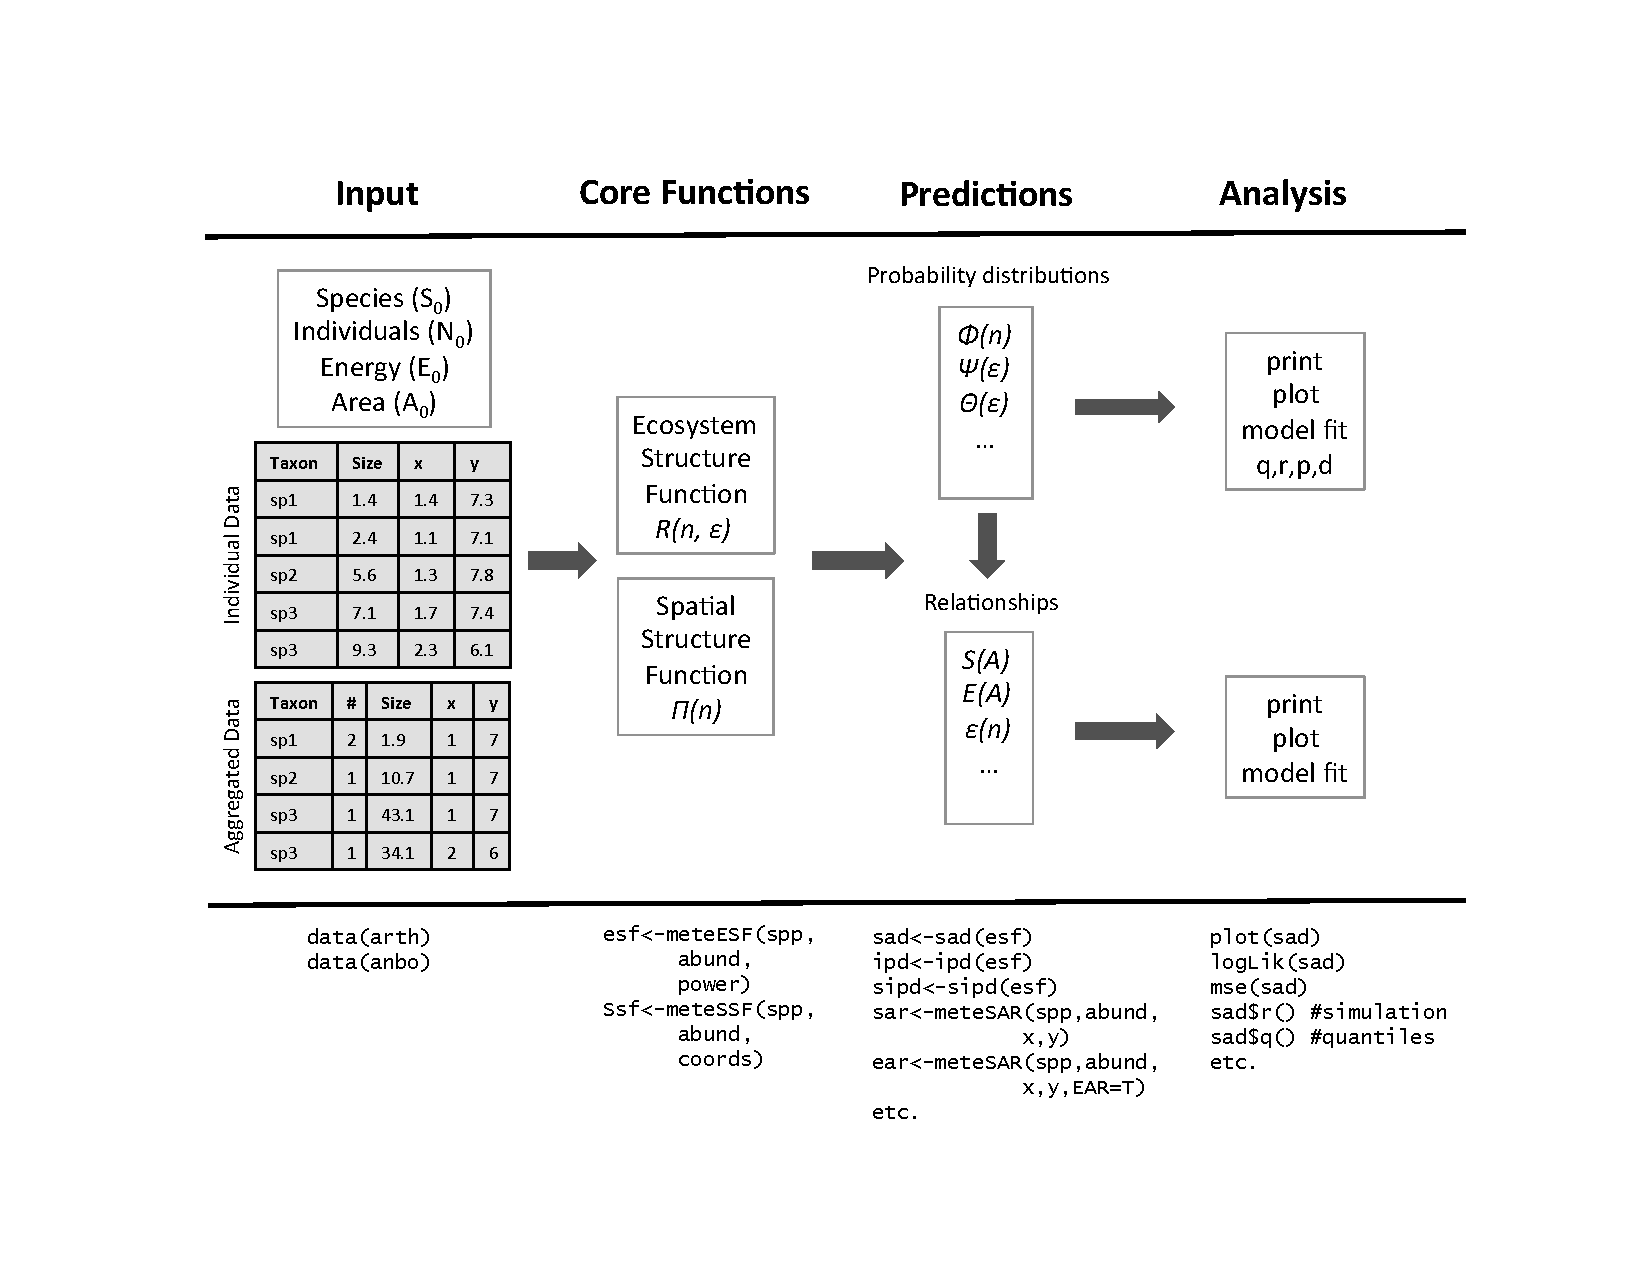
\includegraphics[width=\textwidth]{figs/meteR_workflow.pdf}
    \caption[\texttt{meteR}'s workflow]{\texttt{meteR}'s
      workflow. \texttt{meteR} accepts multiple data types, which are
      used to calculate the core probability distributions from which
      all predictions arise: the \textit{Ecosystem Structure Function}
      (ESF) and the \textit{Spatial Structure Function} (SSF). From
      the ESF and SSF, a variety of macroecological distributions can
      be calculated (see Table \ref{tab:metrics} for
      definitions). Each of these can be plotted or summarized in
      various ways and model fit is readily assessed. Furthermore,
      density, distribution function, quantile function and random
      generation is available for each function, allowing for custom
      plotting, simulation and model evaluation.}
\label{fig:workflow}
\end{center} 
\end{figure}


\begin{figure}[!h] 
  \begin{center}
    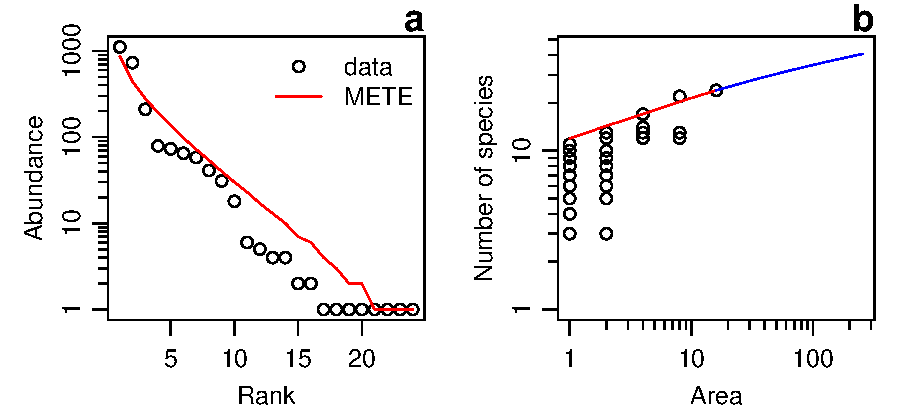
\includegraphics[width=0.75\textwidth]{figs/meteR_MS_v3-anbo_plot}
    \caption[Species abundance distribution and species area
    relationship for the \texttt{anbo} dataset]{Species abundance
      distribution (a) and species area relationship (b) for the
      \texttt{ anbo} dataset. The blue line in (b) depicts the
      upscaled SAR predicted by METE. METE fits the Anza Borrego data
      poorly at increasingly small scales. Understanding such
      systematic deviations from theory could be an opportune area of
      exploration, and initial work suggests that such deviations
      could be an indicator of anthropogenic disturbance (Newman
      \textit{et al.}, in prep.) such as invasive species, which are
      present in the Anza Borrego dataset. Note that we have stylized
      the log axes using custom code not included in \texttt{meteR}.}
\label{fig:anbo}
\end{center} 
\end{figure}


\begin{figure}[!h] 
  \begin{center}
    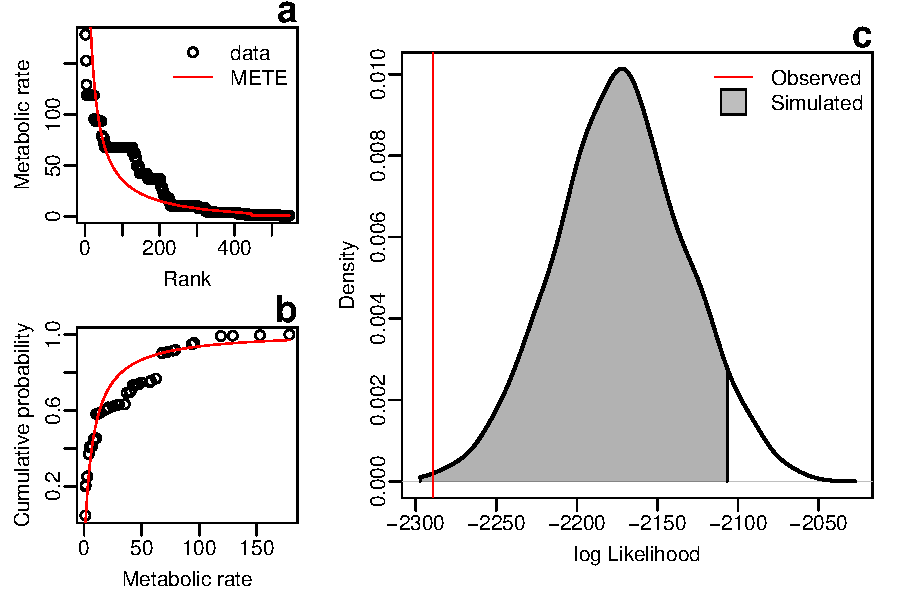
\includegraphics[width=0.75\textwidth]{figs/meteR_MS_v3-arth_plot}
    \caption[Individual power distributions shown]{Individual power
      distributions shown as a rank plot (a) and cumulative density
      plot (b). To evaluate model fit we compare the observed
      likelihood of the data given the METE model (red line in panel
      c) to simulated likelihoods produced by simulated \texttt{nrep}
      communities from the fitted METE object and calculating their
      likelihoods. Thus the simulated distribution represents
      hypothetical likelihoods for datasets obeying METE.}
\label{fig:arth} 
\end{center} 
\end{figure}

\section*{Tables}

%% for raggedright columns
\newcolumntype{L}[1]{>{\raggedright\let\newline\\\arraybackslash\hspace{0pt}}m{#1}}

\begin{table}[!h]
\caption[METE predictions]{METE predictions. Following notational
  conventions in \citet{Harte:2011ut}, $Z$ and $Z_{\Pi}$ are partition
  functions (i.e. to ensure their respective probability distributions
  to sum to 1), $\lambda_1$, $\lambda_2$, and $\lambda_\Pi$ are
  Lagrange multipliers, and commonly used combinations of them include
  $\beta = \lambda_1 + \lambda_2$, $\sigma = \lambda_1 +
  E_0\lambda_2$, and $\gamma=\lambda_{1} + \epsilon \lambda_{2}$.} 
\label{tab:metrics}
\small
\begin{tabular}{L{4cm} p{1.2cm} L{5.4cm} p{2cm} p{2cm}}
  \hline
 Predictions & Acronym & Functional Form & Type & \texttt{meteR} function\\ 
  \hline
      Ecosystem Structure Function & ESF & $R(n,\epsilon | N_0, S_0,E_0) = \frac{1}{Z} e^{-\lambda_1n} e^{-\lambda_2n\epsilon}$  & Core Distribution & \texttt{meteESF} \\ 
	Spatial Structure Function & SSF & $\Pi(n,|n_0, A, A_0) = \frac{1}{Z_\Pi} e^{-\lambda_\Pi n}$& Core Distribution & \texttt{meteSSF} \\
	Distribution of Species Abundance & SAD & $\Phi(n|N_0, S_0)\approx \frac{1}{log\frac{1}{\beta}} \frac{e^{\beta n}}{n}$ & Distribution & \texttt{sad} \\ 
 	Distribution of individual Power across community & IPD & $\Psi(\epsilon|N_0, S_0, E_0)\approx  \lambda_2 \cdot \beta \frac{e^{-\gamma}}{(1-e^{\gamma})^2} $& Distribution & \texttt{ipd} \\
	Distribution of individual Power for species with $n$ individuals & SIPD & $\Theta(\epsilon | n,N_0, S_0, E_0)\approx \lambda_2ne^{-\lambda_2n(\epsilon-1)}$ & Distribution & \texttt{sipd} \\
	Distribution of average (over individuals) metabolic rates over species & SPD & $\nu (\overline{\epsilon} |  N_0, S_0,E_0) \approx \frac{1}{log\frac{1}{\beta}}  \frac{e^{\beta / \lambda_2(\overline{\epsilon} -1)}}{\overline{\epsilon} -1}$ & Distribution & \texttt{spd} \\
	Average individual metabolic rate for species with $n$ individuals & ebar & $\overline{\epsilon}(n | N_0, S_0,E_0) \approx 1 + \frac{1}{n\lambda_2}$ & Relationship & \texttt{ebar} \\
	Species Area Relationship & SAR & $\bar{S}(A) = S_0 \sum_{n=1}^{N_0} \left(1 - \Pi(0 | n)\right) \Phi(n)$ & Relationship & \texttt{meteSAR}, \verb|downscaleSAR|, \verb|upscaleSAR| \\
	Endemics Area Relationship & EAR & $\bar{E}(A) = S_0 \sum_{n=1}^{N_0} \Pi(n | n) \Phi(n)$ & Relationship & \verb|meteSAR|, \verb|downscaleSAR| \\
   \hline
\end{tabular}
\end{table}

